
\documentclass{standalone}
\RequirePackage{esvect}

\usepackage{tikz} % la base
\usetikzlibrary{calc,through,backgrounds}

% Si la compilation de ce fichier échoue avec l'erreur
%	! Package xkeyval Error: `babel' undefined in families `MT',
% commentez la ligne suivante.
\usepackage[babel=true,kerning=true]{microtype} % pour resoudre un
                                % probleme de compatibilite entre
                                % [francais]{babel} et TikZ/PGF.
\usepackage{aeguill}   % Pour forcer une police vectorielle
\pagestyle{empty} % On veut le dessin seul
\begin{document}

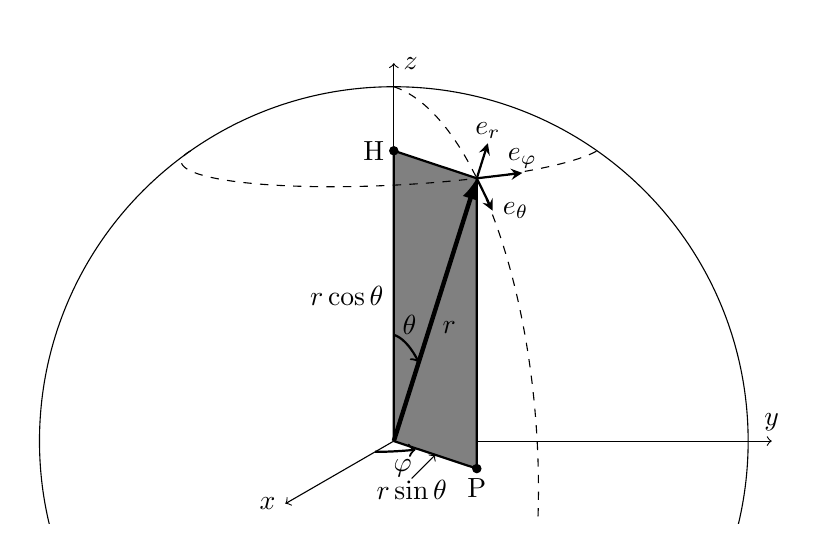
\begin{tikzpicture}[scale=1.5]

%% Les valeurs utiles

%%%%%%%%%%%%%%%%%%%%%%%%%%%%
%% Attention, ne pas faire de modifs directement dans ce fichier .tex
%% car il a été généré à partir d'un fichier .rbtex
%%%%%%%%%%%%%%%%%%%%%%%%%%%%




\pgfsetzvec{\pgfpointxy{-0.30619}{-0.17678}}




  \pgfmathsetmacro{\clipradius}{0.8}



%% Les coordonnées des points principaux
  \coordinate (O)   at (0,0,0) ;
%% Centre de l'ellipse supérieure
  \coordinate (O1)  at (0.0,2.45746,0.0) ;
%% La projection sur le plan horizontal
  \coordinate (P) at (1.10606,0.0,1.31816) ;
%% Le point M et les points suivant les trois axes de base
  \coordinate (M)   at (1.10606,2.45746,1.31816);
  \coordinate (M1t) at (1.23953,2.29813,1.47721);
  \coordinate (M1p) at (1.21674,2.45746,1.21674);
  \coordinate (Mr)  at (1.29041,2.86703,1.53785) ;
  \coordinate (Mrp1)at (1.41953,2.86703,1.41953) ;
  \coordinate (Mrt1)at (1.44612,2.68116,1.72341) ;
  \coordinate (Mt)  at (1.36356,2.12132,1.62503) ;
  \coordinate (Mtr1)at (1.40901,2.19203,1.67919) ;
  \coordinate (Mtp1)at (1.50000,2.12132,1.50000) ;
  \coordinate (Mt1) at (1.23953,2.29813,1.47721) ;
  \coordinate (Mp)  at (1.44313,2.45746,0.93718) ;
  \coordinate (Mpr1)at (1.49123,2.53937,0.96842) ;
  \coordinate (Mpt1)at (1.61726,2.29813,1.05026) ;
  \coordinate (Mp1) at (1.35595,2.45746,1.05939) ;
%% Les coins du volume élémentaire et les petits déplacements alentours
  \coordinate (Apt) at (1.77909,2.12132,1.15535) ;
  \coordinate (A1pt) at (1.83839,2.19203,1.19387) ;
  \coordinate (Ap1t)at (1.67162,2.12132,1.30602) ;
  \coordinate (Apt1)at (1.61726,2.29813,1.05026) ;
  \coordinate (Art) at (1.59082,2.47487,1.89586) ;
  \coordinate (A1rt)at (1.75000,2.47487,1.75000) ;
  \coordinate (Ar1t)at (1.54537,2.40416,1.84170) ;
  \coordinate (Art1)at (1.44612,2.68116,1.72341) ;
  \coordinate (Arp) at (1.68365,2.86703,1.09337) ;
  \coordinate (A1rp)at (1.88680,2.68116,1.22531) ;
  \coordinate (Ar1p)at (1.63554,2.78512,1.06213) ;
  \coordinate (Arp1)at (1.58195,2.86703,1.23595) ;
%% Et le coin opposé et les déplacements alentours
  \coordinate (B)  at (2.07560,2.47487,1.34791) ;
  \coordinate (Br1)at (2.01630,2.40416,1.30940) ;
  \coordinate (Bt1)at (1.88680,2.68116,1.22531) ;
  \coordinate (Bp1)at (1.95023,2.47487,1.52368) ;

%% Le centre du cercle
%  \coordinate (I)   at ($ (M)!0.5!(Mp) $);
  \coordinate (I)   at (barycentric cs:Mt=0.5,Mp=0.5,Mr=0.5);



\def\ELLIPSEUN{\draw [dashed] (0.0,3.00000,0.0) -- (0.0,3.00000,0.0) -- (0.03365,2.99954,0.04011) -- (0.06730,2.99817,0.08020) -- (0.10092,2.99589,0.12028) -- (0.13452,2.99269,0.16031) -- (0.16807,2.98858,0.20030) -- (0.20157,2.98357,0.24022) -- (0.23501,2.97764,0.28007) -- (0.26838,2.97080,0.31984) -- (0.30166,2.96307,0.35951) -- (0.33486,2.95442,0.39907) -- (0.36795,2.94488,0.43850) -- (0.40093,2.93444,0.47781) -- (0.43379,2.92311,0.51697) -- (0.46651,2.91089,0.55597) -- (0.49910,2.89778,0.59480) -- (0.53153,2.88379,0.63345) -- (0.56380,2.86891,0.67191) -- (0.59590,2.85317,0.71016) -- (0.62781,2.83656,0.74820) -- (0.65954,2.81908,0.78601) -- (0.69106,2.80074,0.82358) -- (0.72238,2.78155,0.86090) -- (0.75347,2.76151,0.89795) -- (0.78434,2.74064,0.93474) -- (0.81496,2.71892,0.97123) -- (0.84534,2.69638,1.00744) -- (0.87546,2.67302,1.04333) -- (0.90531,2.64884,1.07891) -- (0.93489,2.62386,1.11416) -- (0.96418,2.59808,1.14907) -- (0.99318,2.57150,1.18363) -- (1.02188,2.54414,1.21783) -- (1.05026,2.51601,1.25165) -- (1.07833,2.48711,1.28510) -- (1.10606,2.45746,1.31816) -- (1.13346,2.42705,1.35081) -- (1.16052,2.39591,1.38305) -- (1.18722,2.36403,1.41487) -- (1.21356,2.33144,1.44626) -- (1.23953,2.29813,1.47721) -- (1.26512,2.26413,1.50771) -- (1.29033,2.22943,1.53775) -- (1.31514,2.19406,1.56732) -- (1.33955,2.15802,1.59642) -- (1.36356,2.12132,1.62503) -- (1.38715,2.08398,1.65314) -- (1.41032,2.04600,1.68075) -- (1.43305,2.00739,1.70785) -- (1.45535,1.96818,1.73442) -- (1.47721,1.92836,1.76047) -- (1.49862,1.88796,1.78599) -- (1.51957,1.84698,1.81095) -- (1.54006,1.80545,1.83537) -- (1.56008,1.76336,1.85923) -- (1.57962,1.72073,1.88252) -- (1.59869,1.67758,1.90524) -- (1.61726,1.63392,1.92738) -- (1.63534,1.58976,1.94893) -- (1.65293,1.54511,1.96988) -- (1.67001,1.50000,1.99024) -- (1.68658,1.45443,2.00999) -- (1.70264,1.40841,2.02913) -- (1.71818,1.36197,2.04765) -- (1.73320,1.31511,2.06555) -- (1.74769,1.26785,2.08282) -- (1.76165,1.22021,2.09945) -- (1.77507,1.17219,2.11544) -- (1.78795,1.12382,2.13079) -- (1.80028,1.07510,2.14549) -- (1.81207,1.02606,2.15954) -- (1.82330,0.97670,2.17293) -- (1.83398,0.92705,2.18565) -- (1.84410,0.87712,2.19772) -- (1.85366,0.82691,2.20911) -- (1.86266,0.77646,2.21983) -- (1.87108,0.72577,2.22987) -- (1.87894,0.67485,2.23923) -- (1.88622,0.62374,2.24791) -- (1.89293,0.57243,2.25591) -- (1.89907,0.52094,2.26322) -- (1.90462,0.46930,2.26984) -- (1.90960,0.41752,2.27577) -- (1.91399,0.36561,2.28100) -- (1.91780,0.31359,2.28554) -- (1.92102,0.26147,2.28939) -- (1.92367,0.20927,2.29254) -- (1.92572,0.15701,2.29498) -- (1.92719,0.10470,2.29673) -- (1.92807,0.05236,2.29778) -- (1.92836,0.0,2.29813) -- (1.92807,-0.05236,2.29778) -- (1.92719,-0.10470,2.29673) -- (1.92572,-0.15701,2.29498) -- (1.92367,-0.20927,2.29254) -- (1.92102,-0.26147,2.28939) -- (1.91780,-0.31359,2.28554) -- (1.91399,-0.36561,2.28100) -- (1.90960,-0.41752,2.27577) -- (1.90462,-0.46930,2.26984) -- (1.89907,-0.52094,2.26322) -- (1.89293,-0.57243,2.25591) -- (1.88622,-0.62374,2.24791) -- (1.87894,-0.67485,2.23923) -- (1.87108,-0.72577,2.22987) -- (1.86266,-0.77646,2.21983) -- (1.85366,-0.82691,2.20911) -- (1.84410,-0.87712,2.19772) -- (1.83398,-0.92705,2.18565) -- (1.82330,-0.97670,2.17293) -- (1.81207,-1.02606,2.15954) -- (1.80028,-1.07510,2.14549) -- (1.78795,-1.12382,2.13079) -- (1.77507,-1.17219,2.11544) -- (1.76165,-1.22021,2.09945) -- (1.74769,-1.26785,2.08282) -- (1.73320,-1.31511,2.06555) -- (1.71818,-1.36197,2.04765) -- (1.70264,-1.40841,2.02913) -- (1.68658,-1.45443,2.00999) -- (1.67001,-1.50000,1.99024) -- (1.65293,-1.54511,1.96988) -- (1.63534,-1.58976,1.94893) -- (1.61726,-1.63392,1.92738) -- (1.59869,-1.67758,1.90524) -- (1.57962,-1.72073,1.88252) -- (1.56008,-1.76336,1.85923) -- (1.54006,-1.80545,1.83537) -- (1.51957,-1.84698,1.81095) -- (1.49862,-1.88796,1.78599) -- (1.47721,-1.92836,1.76047) -- (1.45535,-1.96818,1.73442) -- (1.43305,-2.00739,1.70785) -- (1.41032,-2.04600,1.68075) -- (1.38715,-2.08398,1.65314) -- (1.36356,-2.12132,1.62503) -- (1.33955,-2.15802,1.59642) -- (1.31514,-2.19406,1.56732) -- (1.29033,-2.22943,1.53775) -- (1.26512,-2.26413,1.50771) -- (1.23953,-2.29813,1.47721) -- (1.21356,-2.33144,1.44626) -- (1.18722,-2.36403,1.41487) -- (1.16052,-2.39591,1.38305) -- (1.13346,-2.42705,1.35081);
}

\def\ELLIPSEDEUX{\draw [dashed] (0.0,3.00000,0.0) -- (0.0,3.00000,0.0) -- (0.04391,2.99954,0.02852) -- (0.08781,2.99817,0.05702) -- (0.13168,2.99589,0.08551) -- (0.17551,2.99269,0.11398) -- (0.21928,2.98858,0.14241) -- (0.26299,2.98357,0.17079) -- (0.30662,2.97764,0.19912) -- (0.35016,2.97080,0.22740) -- (0.39359,2.96307,0.25560) -- (0.43690,2.95442,0.28373) -- (0.48008,2.94488,0.31177) -- (0.52311,2.93444,0.33971) -- (0.56598,2.92311,0.36755) -- (0.60868,2.91089,0.39528) -- (0.65119,2.89778,0.42289) -- (0.69351,2.88379,0.45037) -- (0.73561,2.86891,0.47771) -- (0.77749,2.85317,0.50491) -- (0.81913,2.83656,0.53195) -- (0.86053,2.81908,0.55883) -- (0.90166,2.80074,0.58554) -- (0.94251,2.78155,0.61208) -- (0.98308,2.76151,0.63842) -- (1.02335,2.74064,0.66457) -- (1.06331,2.71892,0.69052) -- (1.10295,2.69638,0.71626) -- (1.14225,2.67302,0.74178) -- (1.18120,2.64884,0.76708) -- (1.21979,2.62386,0.79214) -- (1.25801,2.59808,0.81696) -- (1.29584,2.57150,0.84153) -- (1.33328,2.54414,0.86584) -- (1.37032,2.51601,0.88990) -- (1.40694,2.48711,0.91367) -- (1.44313,2.45746,0.93718) -- (1.47887,2.42705,0.96039) -- (1.51417,2.39591,0.98332) -- (1.54901,2.36403,1.00594) -- (1.58338,2.33144,1.02826) -- (1.61726,2.29813,1.05026) -- (1.65065,2.26413,1.07195) -- (1.68354,2.22943,1.09330) -- (1.71592,2.19406,1.11433) -- (1.74777,2.15802,1.13501) -- (1.77909,2.12132,1.15535) -- (1.80987,2.08398,1.17534) -- (1.84009,2.04600,1.19497) -- (1.86976,2.00739,1.21424) -- (1.89886,1.96818,1.23313) -- (1.92738,1.92836,1.25165) -- (1.95531,1.88796,1.26979) -- (1.98264,1.84698,1.28754) -- (2.00938,1.80545,1.30490) -- (2.03550,1.76336,1.32187) -- (2.06100,1.72073,1.33843) -- (2.08587,1.67758,1.35458) -- (2.11010,1.63392,1.37032) -- (2.13370,1.58976,1.38564) -- (2.15664,1.54511,1.40054) -- (2.17893,1.50000,1.41501) -- (2.20055,1.45443,1.42906) -- (2.22151,1.40841,1.44266) -- (2.24178,1.36197,1.45583) -- (2.26138,1.31511,1.46855) -- (2.28028,1.26785,1.48083) -- (2.29849,1.22021,1.49266) -- (2.31600,1.17219,1.50403) -- (2.33281,1.12382,1.51494) -- (2.34890,1.07510,1.52539) -- (2.36428,1.02606,1.53538) -- (2.37894,0.97670,1.54490) -- (2.39287,0.92705,1.55395) -- (2.40607,0.87712,1.56252) -- (2.41855,0.82691,1.57062) -- (2.43028,0.77646,1.57824) -- (2.44128,0.72577,1.58538) -- (2.45153,0.67485,1.59204) -- (2.46103,0.62374,1.59821) -- (2.46979,0.57243,1.60390) -- (2.47779,0.52094,1.60909) -- (2.48504,0.46930,1.61380) -- (2.49153,0.41752,1.61802) -- (2.49726,0.36561,1.62174) -- (2.50223,0.31359,1.62497) -- (2.50644,0.26147,1.62770) -- (2.50988,0.20927,1.62994) -- (2.51256,0.15701,1.63168) -- (2.51448,0.10470,1.63292) -- (2.51563,0.05236,1.63367) -- (2.51601,0.0,1.63392) -- (2.51563,-0.05236,1.63367) -- (2.51448,-0.10470,1.63292) -- (2.51256,-0.15701,1.63168) -- (2.50988,-0.20927,1.62994) -- (2.50644,-0.26147,1.62770) -- (2.50223,-0.31359,1.62497) -- (2.49726,-0.36561,1.62174) -- (2.49153,-0.41752,1.61802) -- (2.48504,-0.46930,1.61380) -- (2.47779,-0.52094,1.60909) -- (2.46979,-0.57243,1.60390) -- (2.46103,-0.62374,1.59821) -- (2.45153,-0.67485,1.59204) -- (2.44128,-0.72577,1.58538) -- (2.43028,-0.77646,1.57824) -- (2.41855,-0.82691,1.57062) -- (2.40607,-0.87712,1.56252) -- (2.39287,-0.92705,1.55395) -- (2.37894,-0.97670,1.54490) -- (2.36428,-1.02606,1.53538) -- (2.34890,-1.07510,1.52539) -- (2.33281,-1.12382,1.51494) -- (2.31600,-1.17219,1.50403) -- (2.29849,-1.22021,1.49266) -- (2.28028,-1.26785,1.48083) -- (2.26138,-1.31511,1.46855) -- (2.24178,-1.36197,1.45583) -- (2.22151,-1.40841,1.44266) -- (2.20055,-1.45443,1.42906) -- (2.17893,-1.50000,1.41501) -- (2.15664,-1.54511,1.40054) -- (2.13370,-1.58976,1.38564) -- (2.11010,-1.63392,1.37032) -- (2.08587,-1.67758,1.35458) -- (2.06100,-1.72073,1.33843) -- (2.03550,-1.76336,1.32187) -- (2.00938,-1.80545,1.30490) -- (1.98264,-1.84698,1.28754) -- (1.95531,-1.88796,1.26979) -- (1.92738,-1.92836,1.25165) -- (1.89886,-1.96818,1.23313) -- (1.86976,-2.00739,1.21424) -- (1.84009,-2.04600,1.19497) -- (1.80987,-2.08398,1.17534) -- (1.77909,-2.12132,1.15535) -- (1.74777,-2.15802,1.13501) -- (1.71592,-2.19406,1.11433) -- (1.68354,-2.22943,1.09330) -- (1.65065,-2.26413,1.07195) -- (1.61726,-2.29813,1.05026) -- (1.58338,-2.33144,1.02826) -- (1.54901,-2.36403,1.00594) -- (1.51417,-2.39591,0.98332) -- (1.47887,-2.42705,0.96039);
}

\def\ELLIPSETROIS{\draw [dashed] (-1.72073,2.45746,0.0) -- (-1.72047,2.45746,0.03003) -- (-1.71968,2.45746,0.06005) -- (-1.71837,2.45746,0.09006) -- (-1.71654,2.45746,0.12003) -- (-1.71418,2.45746,0.14997) -- (-1.71130,2.45746,0.17987) -- (-1.70790,2.45746,0.20970) -- (-1.70398,2.45746,0.23948) -- (-1.69954,2.45746,0.26918) -- (-1.69459,2.45746,0.29880) -- (-1.68911,2.45746,0.32833) -- (-1.68313,2.45746,0.35776) -- (-1.67663,2.45746,0.38708) -- (-1.66962,2.45746,0.41628) -- (-1.66210,2.45746,0.44536) -- (-1.65407,2.45746,0.47430) -- (-1.64554,2.45746,0.50309) -- (-1.63651,2.45746,0.53173) -- (-1.62698,2.45746,0.56021) -- (-1.61696,2.45746,0.58852) -- (-1.60644,2.45746,0.61665) -- (-1.59543,2.45746,0.64460) -- (-1.58394,2.45746,0.67234) -- (-1.57196,2.45746,0.69988) -- (-1.55951,2.45746,0.72721) -- (-1.54658,2.45746,0.75432) -- (-1.53318,2.45746,0.78119) -- (-1.51931,2.45746,0.80783) -- (-1.50498,2.45746,0.83423) -- (-1.49020,2.45746,0.86036) -- (-1.47495,2.45746,0.88624) -- (-1.45926,2.45746,0.91185) -- (-1.44313,2.45746,0.93718) -- (-1.42655,2.45746,0.96222) -- (-1.40954,2.45746,0.98697) -- (-1.39210,2.45746,1.01142) -- (-1.37424,2.45746,1.03556) -- (-1.35595,2.45746,1.05939) -- (-1.33726,2.45746,1.08289) -- (-1.31816,2.45746,1.10606) -- (-1.29865,2.45746,1.12890) -- (-1.27875,2.45746,1.15139) -- (-1.25846,2.45746,1.17353) -- (-1.23779,2.45746,1.19532) -- (-1.21674,2.45746,1.21674) -- (-1.19532,2.45746,1.23779) -- (-1.17353,2.45746,1.25846) -- (-1.15139,2.45746,1.27875) -- (-1.12890,2.45746,1.29865) -- (-1.10606,2.45746,1.31816) -- (-1.08289,2.45746,1.33726) -- (-1.05939,2.45746,1.35595) -- (-1.03556,2.45746,1.37424) -- (-1.01142,2.45746,1.39210) -- (-0.98697,2.45746,1.40954) -- (-0.96222,2.45746,1.42655) -- (-0.93718,2.45746,1.44313) -- (-0.91185,2.45746,1.45926) -- (-0.88624,2.45746,1.47495) -- (-0.86036,2.45746,1.49020) -- (-0.83423,2.45746,1.50498) -- (-0.80783,2.45746,1.51931) -- (-0.78119,2.45746,1.53318) -- (-0.75432,2.45746,1.54658) -- (-0.72721,2.45746,1.55951) -- (-0.69988,2.45746,1.57196) -- (-0.67234,2.45746,1.58394) -- (-0.64460,2.45746,1.59543) -- (-0.61665,2.45746,1.60644) -- (-0.58852,2.45746,1.61696) -- (-0.56021,2.45746,1.62698) -- (-0.53173,2.45746,1.63651) -- (-0.50309,2.45746,1.64554) -- (-0.47430,2.45746,1.65407) -- (-0.44536,2.45746,1.66210) -- (-0.41628,2.45746,1.66962) -- (-0.38708,2.45746,1.67663) -- (-0.35776,2.45746,1.68313) -- (-0.32833,2.45746,1.68911) -- (-0.29880,2.45746,1.69459) -- (-0.26918,2.45746,1.69954) -- (-0.23948,2.45746,1.70398) -- (-0.20970,2.45746,1.70790) -- (-0.17987,2.45746,1.71130) -- (-0.14997,2.45746,1.71418) -- (-0.12003,2.45746,1.71654) -- (-0.09006,2.45746,1.71837) -- (-0.06005,2.45746,1.71968) -- (-0.03003,2.45746,1.72047) -- (0.0,2.45746,1.72073) -- (0.03003,2.45746,1.72047) -- (0.06005,2.45746,1.71968) -- (0.09006,2.45746,1.71837) -- (0.12003,2.45746,1.71654) -- (0.14997,2.45746,1.71418) -- (0.17987,2.45746,1.71130) -- (0.20970,2.45746,1.70790) -- (0.23948,2.45746,1.70398) -- (0.26918,2.45746,1.69954) -- (0.29880,2.45746,1.69459) -- (0.32833,2.45746,1.68911) -- (0.35776,2.45746,1.68313) -- (0.38708,2.45746,1.67663) -- (0.41628,2.45746,1.66962) -- (0.44536,2.45746,1.66210) -- (0.47430,2.45746,1.65407) -- (0.50309,2.45746,1.64554) -- (0.53173,2.45746,1.63651) -- (0.56021,2.45746,1.62698) -- (0.58852,2.45746,1.61696) -- (0.61665,2.45746,1.60644) -- (0.64460,2.45746,1.59543) -- (0.67234,2.45746,1.58394) -- (0.69988,2.45746,1.57196) -- (0.72721,2.45746,1.55951) -- (0.75432,2.45746,1.54658) -- (0.78119,2.45746,1.53318) -- (0.80783,2.45746,1.51931) -- (0.83423,2.45746,1.50498) -- (0.86036,2.45746,1.49020) -- (0.88624,2.45746,1.47495) -- (0.91185,2.45746,1.45926) -- (0.93718,2.45746,1.44313) -- (0.96222,2.45746,1.42655) -- (0.98697,2.45746,1.40954) -- (1.01142,2.45746,1.39210) -- (1.03556,2.45746,1.37424) -- (1.05939,2.45746,1.35595) -- (1.08289,2.45746,1.33726) -- (1.10606,2.45746,1.31816) -- (1.12890,2.45746,1.29865) -- (1.15139,2.45746,1.27875) -- (1.17353,2.45746,1.25846) -- (1.19532,2.45746,1.23779) -- (1.21674,2.45746,1.21674) -- (1.23779,2.45746,1.19532) -- (1.25846,2.45746,1.17353) -- (1.27875,2.45746,1.15139) -- (1.29865,2.45746,1.12890) -- (1.31816,2.45746,1.10606) -- (1.33726,2.45746,1.08289) -- (1.35595,2.45746,1.05939) -- (1.37424,2.45746,1.03556) -- (1.39210,2.45746,1.01142) -- (1.40954,2.45746,0.98697) -- (1.42655,2.45746,0.96222) -- (1.44313,2.45746,0.93718) -- (1.45926,2.45746,0.91185) -- (1.47495,2.45746,0.88624) -- (1.49020,2.45746,0.86036) -- (1.50498,2.45746,0.83423) -- (1.51931,2.45746,0.80783) -- (1.53318,2.45746,0.78119) -- (1.54658,2.45746,0.75432) -- (1.55951,2.45746,0.72721) -- (1.57196,2.45746,0.69988) -- (1.58394,2.45746,0.67234) -- (1.59543,2.45746,0.64460) -- (1.60644,2.45746,0.61665) -- (1.61696,2.45746,0.58852) -- (1.62698,2.45746,0.56021) -- (1.63651,2.45746,0.53173) -- (1.64554,2.45746,0.50309) -- (1.65407,2.45746,0.47430) -- (1.66210,2.45746,0.44536) -- (1.66962,2.45746,0.41628) -- (1.67663,2.45746,0.38708) -- (1.68313,2.45746,0.35776) -- (1.68911,2.45746,0.32833) -- (1.69459,2.45746,0.29880) -- (1.69954,2.45746,0.26918) -- (1.70398,2.45746,0.23948) -- (1.70790,2.45746,0.20970) -- (1.71130,2.45746,0.17987) -- (1.71418,2.45746,0.14997) -- (1.71654,2.45746,0.12003) -- (1.71837,2.45746,0.09006) -- (1.71968,2.45746,0.06005) -- (1.72047,2.45746,0.03003) -- (1.72073,2.45746,0.0);
}

\def\ELLIPSEQUATRE{\draw [dashed] (-2.12132,2.12132,0.0) -- (-2.12100,2.12132,0.03702) -- (-2.12003,2.12132,0.07403) -- (-2.11841,2.12132,0.11102) -- (-2.11615,2.12132,0.14798) -- (-2.11325,2.12132,0.18489) -- (-2.10970,2.12132,0.22174) -- (-2.10551,2.12132,0.25852) -- (-2.10068,2.12132,0.29523) -- (-2.09520,2.12132,0.33185) -- (-2.08909,2.12132,0.36836) -- (-2.08235,2.12132,0.40477) -- (-2.07496,2.12132,0.44105) -- (-2.06695,2.12132,0.47719) -- (-2.05831,2.12132,0.51319) -- (-2.04904,2.12132,0.54904) -- (-2.03914,2.12132,0.58472) -- (-2.02863,2.12132,0.62021) -- (-2.01750,2.12132,0.65552) -- (-2.00575,2.12132,0.69063) -- (-1.99339,2.12132,0.72553) -- (-1.98042,2.12132,0.76021) -- (-1.96685,2.12132,0.79466) -- (-1.95269,2.12132,0.82887) -- (-1.93792,2.12132,0.86282) -- (-1.92257,2.12132,0.89651) -- (-1.90663,2.12132,0.92993) -- (-1.89011,2.12132,0.96306) -- (-1.87301,2.12132,0.99590) -- (-1.85535,2.12132,1.02844) -- (-1.83712,2.12132,1.06066) -- (-1.81833,2.12132,1.09256) -- (-1.79898,2.12132,1.12413) -- (-1.77909,2.12132,1.15535) -- (-1.75865,2.12132,1.18623) -- (-1.73768,2.12132,1.21674) -- (-1.71618,2.12132,1.24688) -- (-1.69416,2.12132,1.27664) -- (-1.67162,2.12132,1.30602) -- (-1.64858,2.12132,1.33499) -- (-1.62503,2.12132,1.36356) -- (-1.60098,2.12132,1.39171) -- (-1.57645,2.12132,1.41944) -- (-1.55144,2.12132,1.44674) -- (-1.52595,2.12132,1.47359) -- (-1.50000,2.12132,1.50000) -- (-1.47359,2.12132,1.52595) -- (-1.44674,2.12132,1.55144) -- (-1.41944,2.12132,1.57645) -- (-1.39171,2.12132,1.60098) -- (-1.36356,2.12132,1.62503) -- (-1.33499,2.12132,1.64858) -- (-1.30602,2.12132,1.67162) -- (-1.27664,2.12132,1.69416) -- (-1.24688,2.12132,1.71618) -- (-1.21674,2.12132,1.73768) -- (-1.18623,2.12132,1.75865) -- (-1.15535,2.12132,1.77909) -- (-1.12413,2.12132,1.79898) -- (-1.09256,2.12132,1.81833) -- (-1.06066,2.12132,1.83712) -- (-1.02844,2.12132,1.85535) -- (-0.99590,2.12132,1.87301) -- (-0.96306,2.12132,1.89011) -- (-0.92993,2.12132,1.90663) -- (-0.89651,2.12132,1.92257) -- (-0.86282,2.12132,1.93792) -- (-0.82887,2.12132,1.95269) -- (-0.79466,2.12132,1.96685) -- (-0.76021,2.12132,1.98042) -- (-0.72553,2.12132,1.99339) -- (-0.69063,2.12132,2.00575) -- (-0.65552,2.12132,2.01750) -- (-0.62021,2.12132,2.02863) -- (-0.58472,2.12132,2.03914) -- (-0.54904,2.12132,2.04904) -- (-0.51319,2.12132,2.05831) -- (-0.47719,2.12132,2.06695) -- (-0.44105,2.12132,2.07496) -- (-0.40477,2.12132,2.08235) -- (-0.36836,2.12132,2.08909) -- (-0.33185,2.12132,2.09520) -- (-0.29523,2.12132,2.10068) -- (-0.25852,2.12132,2.10551) -- (-0.22174,2.12132,2.10970) -- (-0.18489,2.12132,2.11325) -- (-0.14798,2.12132,2.11615) -- (-0.11102,2.12132,2.11841) -- (-0.07403,2.12132,2.12003) -- (-0.03702,2.12132,2.12100) -- (0.0,2.12132,2.12132) -- (0.03702,2.12132,2.12100) -- (0.07403,2.12132,2.12003) -- (0.11102,2.12132,2.11841) -- (0.14798,2.12132,2.11615) -- (0.18489,2.12132,2.11325) -- (0.22174,2.12132,2.10970) -- (0.25852,2.12132,2.10551) -- (0.29523,2.12132,2.10068) -- (0.33185,2.12132,2.09520) -- (0.36836,2.12132,2.08909) -- (0.40477,2.12132,2.08235) -- (0.44105,2.12132,2.07496) -- (0.47719,2.12132,2.06695) -- (0.51319,2.12132,2.05831) -- (0.54904,2.12132,2.04904) -- (0.58472,2.12132,2.03914) -- (0.62021,2.12132,2.02863) -- (0.65552,2.12132,2.01750) -- (0.69063,2.12132,2.00575) -- (0.72553,2.12132,1.99339) -- (0.76021,2.12132,1.98042) -- (0.79466,2.12132,1.96685) -- (0.82887,2.12132,1.95269) -- (0.86282,2.12132,1.93792) -- (0.89651,2.12132,1.92257) -- (0.92993,2.12132,1.90663) -- (0.96306,2.12132,1.89011) -- (0.99590,2.12132,1.87301) -- (1.02844,2.12132,1.85535) -- (1.06066,2.12132,1.83712) -- (1.09256,2.12132,1.81833) -- (1.12413,2.12132,1.79898) -- (1.15535,2.12132,1.77909) -- (1.18623,2.12132,1.75865) -- (1.21674,2.12132,1.73768) -- (1.24688,2.12132,1.71618) -- (1.27664,2.12132,1.69416) -- (1.30602,2.12132,1.67162) -- (1.33499,2.12132,1.64858) -- (1.36356,2.12132,1.62503) -- (1.39171,2.12132,1.60098) -- (1.41944,2.12132,1.57645) -- (1.44674,2.12132,1.55144) -- (1.47359,2.12132,1.52595) -- (1.50000,2.12132,1.50000) -- (1.52595,2.12132,1.47359) -- (1.55144,2.12132,1.44674) -- (1.57645,2.12132,1.41944) -- (1.60098,2.12132,1.39171) -- (1.62503,2.12132,1.36356) -- (1.64858,2.12132,1.33499) -- (1.67162,2.12132,1.30602) -- (1.69416,2.12132,1.27664) -- (1.71618,2.12132,1.24688) -- (1.73768,2.12132,1.21674) -- (1.75865,2.12132,1.18623) -- (1.77909,2.12132,1.15535) -- (1.79898,2.12132,1.12413) -- (1.81833,2.12132,1.09256) -- (1.83712,2.12132,1.06066) -- (1.85535,2.12132,1.02844) -- (1.87301,2.12132,0.99590) -- (1.89011,2.12132,0.96306) -- (1.90663,2.12132,0.92993) -- (1.92257,2.12132,0.89651) -- (1.93792,2.12132,0.86282) -- (1.95269,2.12132,0.82887) -- (1.96685,2.12132,0.79466) -- (1.98042,2.12132,0.76021) -- (1.99339,2.12132,0.72553) -- (2.00575,2.12132,0.69063) -- (2.01750,2.12132,0.65552) -- (2.02863,2.12132,0.62021) -- (2.03914,2.12132,0.58472) -- (2.04904,2.12132,0.54904) -- (2.05831,2.12132,0.51319) -- (2.06695,2.12132,0.47719) -- (2.07496,2.12132,0.44105) -- (2.08235,2.12132,0.40477) -- (2.08909,2.12132,0.36836) -- (2.09520,2.12132,0.33185) -- (2.10068,2.12132,0.29523) -- (2.10551,2.12132,0.25852) -- (2.10970,2.12132,0.22174) -- (2.11325,2.12132,0.18489) -- (2.11615,2.12132,0.14798) -- (2.11841,2.12132,0.11102) -- (2.12003,2.12132,0.07403) -- (2.12100,2.12132,0.03702) -- (2.12132,2.12132,0.0);
}



\def\DPHI{
	\draw [<->,thick] (0.33182,2.45746,0.39545) -- (0.34467,2.45746,0.38429) -- (0.35715,2.45746,0.37272) -- (0.36924,2.45746,0.36075) -- (0.38093,2.45746,0.34838) -- (0.39221,2.45746,0.33564) -- (0.40306,2.45746,0.32253) -- (0.41347,2.45746,0.30907) -- (0.42344,2.45746,0.29527) -- (0.43294,2.45746,0.28115) ;
	\draw (0.38663,2.45746,0.34206) node [above] {$\dd\varphi$} ;
}

\def\DTHETA{
	\draw [<->,thick] (0.89591,1.99054,1.06771) -- (0.92055,1.96314,1.09707) -- (0.94485,1.93500,1.12603) -- (0.96879,1.90613,1.15456) -- (0.99237,1.87655,1.18266) -- (1.01557,1.84626,1.21031) -- (1.03839,1.81527,1.23751) -- (1.06082,1.78360,1.26424) -- (1.08286,1.75127,1.29050) -- (1.10448,1.71827,1.31627);
	\draw (0.95683,1.88260,1.14031) node [above right=-3pt] {$\dd\theta$} ;
}

\def\PHI{
	\draw [->,thick] (0.0,0.0,0.51622) -- (0.00680,0.0,0.51617) -- (0.01360,0.0,0.51604) -- (0.02040,0.0,0.51582) -- (0.02720,0.0,0.51550) -- (0.03399,0.0,0.51510) -- (0.04078,0.0,0.51461) -- (0.04756,0.0,0.51402) -- (0.05433,0.0,0.51335) -- (0.06109,0.0,0.51259) -- (0.06784,0.0,0.51174) -- (0.07457,0.0,0.51080) -- (0.08130,0.0,0.50978) -- (0.08801,0.0,0.50866) -- (0.09471,0.0,0.50746) -- (0.10139,0.0,0.50616) -- (0.10805,0.0,0.50478) -- (0.11469,0.0,0.50332) -- (0.12131,0.0,0.50176) -- (0.12792,0.0,0.50012) -- (0.13450,0.0,0.49839) -- (0.14105,0.0,0.49657) -- (0.14758,0.0,0.49467) -- (0.15409,0.0,0.49268) -- (0.16057,0.0,0.49061) -- (0.16702,0.0,0.48845) -- (0.17344,0.0,0.48621) -- (0.17984,0.0,0.48388) -- (0.18620,0.0,0.48147) -- (0.19253,0.0,0.47897) -- (0.19882,0.0,0.47639) -- (0.20508,0.0,0.47373) -- (0.21131,0.0,0.47099) -- (0.21750,0.0,0.46816) -- (0.22365,0.0,0.46526) -- (0.22976,0.0,0.46227) -- (0.23583,0.0,0.45920) -- (0.24186,0.0,0.45605) -- (0.24785,0.0,0.45283) -- (0.25380,0.0,0.44952) -- (0.25970,0.0,0.44614) -- (0.26556,0.0,0.44268) -- (0.27137,0.0,0.43914) -- (0.27713,0.0,0.43552) -- (0.28285,0.0,0.43183) -- (0.28851,0.0,0.42807) -- (0.29413,0.0,0.42423) -- (0.29969,0.0,0.42032) -- (0.30521,0.0,0.41633) -- (0.31067,0.0,0.41227) ;
	\draw (0.47082,0.0,1.29357) node {$\varphi$} ;
}

\def\THETA{
	\draw [->,thick] (0.0,0.90000,0.0) -- (0.03924,0.89793,0.04676) -- (0.07829,0.89172,0.09330) -- (0.11698,0.88141,0.13942) -- (0.15514,0.86703,0.18489) -- (0.19258,0.84867,0.22951) -- (0.22914,0.82639,0.27307) -- (0.26463,0.80032,0.31538) -- (0.29892,0.77055,0.35623) -- (0.33182,0.73724,0.39545);
	\draw (0.20875,1.03001,0.24878) node {$\theta$} ;
}

\def\VER{
	\draw [thick, -stealth, shift=(M)] (0,0,0) -- (0.14748,0.32766,0.17575) 
	node [above=-2pt] {$\vv{e_r}$};
}

\def\VETHETA{
	\draw [thick, -stealth, shift=(M)] (0,0,0) -- (0.21062,-0.22943,0.25100) 
	node [right] {$\vv{e_\theta}$};
}

\def\VEPHI{
	\draw [thick, -stealth, shift=(M)] (0,0,0) -- (0.30642,0.0,-0.25712) 
	node [above=-2pt] {$\vv{e_\varphi}$};
}


\clip  (-3.1,-0.7) rectangle (3.5,3.5);

%% Les axes

\draw [->] (O) -- (0,0,3)  node [left] {$x$} ;
\draw [->] (O) -- (3.2,0,0)  node [above] {$y$} ;
\draw [->] (O) -- (0,3.2,0)  node [right] {$z$} ;

% Le cercle

\draw (O) circle (3) ;

\filldraw [thick, fill=gray] (O) -- (O1) node [pos=0.5,left] {$r\cos\theta$} 
		-- (M) 		
		-- (P) -- (O) 
		;

\coordinate (Mi) at ($ 0.5*(P) + 0.5*(O)$);
\coordinate (Mib) at ($ (Mi) + (-0.2,-0.2) $);

\draw [<-] (Mi) -- (Mib)
		node [below=-3pt] {$ r\sin\theta$} ;

% Position des points principaux
%  \filldraw[black] (M) circle(1pt) node [left] {$M$} ;
  \filldraw[black] (O1)circle(1pt) node [left] {$\mathrm{H}$} ;
  \filldraw[black] (P) circle(1pt) node [below] {$\mathrm{P}$} ;

%% Les lignes d'angles
  \draw [ultra thick,-latex] (O) -- (M) node [pos=0.5,below] {$\quad r$};


%% Les ellipses des construction
    
  \ELLIPSEUN
%  \ELLIPSEDEUX
  \ELLIPSETROIS
%  \ELLIPSEQUATRE

%% Vecteurs
\VER
\VETHETA
\VEPHI

%  \draw (0,-3) -- (0,3) ;

%% Angles

\THETA
\PHI


\end{tikzpicture}

\end{document}

